\documentclass[a4paper]{article}

\usepackage[english]{babel}
\usepackage[utf8x]{inputenc}
\usepackage{amsmath}
\usepackage{graphicx}
\usepackage[colorinlistoftodos]{todonotes}
\usepackage[margin=1.2in]{geometry}
\usepackage{minted}
\usepackage{graphicx}
\usepackage{svg}
\usepackage{hyperref}

\usepackage{titlesec}
\titlespacing*{\section}{0pt}{3.5ex plus 1ex minus .2ex}{2.6ex plus .2ex}

\newgeometry{margin=1in}
\begin{document}
\begin{titlepage}
    \centering
    \vspace*{1in}
    
    {\Large \textbf{Python Project 2:}} \\
    \vspace{0.4in}
    {\huge \textbf{Weather Data Analysis}} \\
    \vspace{0.6in}
    \includesvg[width=0.4\textwidth]{cusat.svg} \\
    \vspace{0.8in}
    
    {\large Submitted by} \\
    \vspace{0.2in}
    {\large \underline{Group - 5}} \\
    \vspace{0.2in}
    
    % This table centers the block of names but left-aligns the text within it
    {\large
    \begin{tabular}{rl}
         2. & \textbf{Aaromal A (24101880)} \\
        15. & \textbf{Alfin Francis (24101006)} \\
        33. & \textbf{Devanarayanan C R (24101115)} \\
        39. & \textbf{G Govardan (24102775)} \\
        49. & \textbf{Ivana Anto (24101562)}
    \end{tabular}}
    
    \vfill
\end{titlepage}
\restoregeometry % Returns margins to 1.2in for the rest of the report
\newpage

\title{Weather Data Analysis}
\author{}
\date{5 February, 2026}
\maketitle

\section*{Aim}

To develop a Python-based weather data analysis application that fetches real-time weather data from the OpenWeatherMap API, processes and cleans the data by handling missing values and duplicates, and visualizes temperature trends and relationships between weather parameters using interactive graphical plots.

\section*{Tools Used}
\begin{itemize}
    \item \textbf{Python 3.14} - Programming language
    \item \textbf{Jupyter Notebook} - Interactive development environment
    \item \textbf{tkinter} - GUI framework for creating the application interface
    \item \textbf{pandas} - Data manipulation and analysis library
    \item \textbf{matplotlib} - Data visualization and plotting library
    \item \textbf{requests} - HTTP library for API communication
    \item \textbf{json} - JSON data parsing and manipulation
    \item \textbf{numpy} - Numerical computing library
    \item \textbf{OpenWeatherMapAPI} - for real-time weather forecast (data source)
\end{itemize}

\vspace{10pt}

\section*{Data Source - OpenWeatherMap API}

OpenWeatherMap is a popular weather data service that provides current weather data, forecasts, and historical weather information through a RESTful API. The API offers various endpoints for different types of weather data.

\subsection*{API Endpoint :}
For this project, we use the \textbf{5-day/3-hour Forecast API}:
\begin{verbatim}
https://api.openweathermap.org/data/2.5/forecast
\end{verbatim}

\subsection*{API Parameters :}
\begin{itemize}
    \item \texttt{q} - City name (e.g., "London", "New York")
    \item \texttt{appid} - API key for authentication
    \item \texttt{units} - Unit system (metric for Celsius, imperial for Fahrenheit)
\end{itemize}

\subsection*{API Response Structure :}
The API returns JSON data containing:
\begin{itemize}
    \item City information (name, country, coordinates)
    \item List of weather forecasts (40 data points over 5 days)
    \item For each forecast: timestamp, temperature, humidity, pressure, weather description, wind speed
\end{itemize}

\subsection*{Basic API Usage :}
\begin{minted}[frame=lines, framesep=2mm, baselinestretch=1.2, fontsize=\footnotesize]{python}
import requests as res

with open("./config/wthrkey", "r") as fp:
    API_KEY = fp.read().strip()

CITY = "Kochi"
URL = f"http://api.openweathermap.org/data/2.5/weather?q={CITY}&appid={KEY}&units=metric"
print(res.get(URL).json())

''' 
output :
{'coord': {'lon': 76.2602, 'lat': 9.9399}, 'weather': [{'id': 802, 'main': 'Clouds', 'description':
'scattered clouds', 'icon': '03d'}], 'base': 'stations', 'main': {'temp': 25.28, 'feels_like': 25.98,
'temp_min': 25.28, 'temp_max': 25.28, 'pressure': 1012, 'humidity': 81, 'sea_level': 1012, 'grnd_level':
1012}, 'visibility': 10000, 'wind': {'speed': 2.24, 'deg': 37, 'gust': 2.4}, 'clouds': {'all': 33}, 'dt':
1772420078, 'sys': {'country': 'IN', 'sunrise': 1772413747, 'sunset': 1772456736}, 'timezone': 19800,
'id': 1273874, 'name': 'Kochi', 'cod': 200}
'''
\end{minted}

\vspace{20pt}

\section*{Source Code}

\begin{minted}[frame=lines, framesep=2mm, baselinestretch=1.2, fontsize=\footnotesize, linenos]{python}
import requests
import pandas as pd
import numpy as np
import tkinter as tk
from tkinter import messagebox
from matplotlib.figure import Figure
from matplotlib.backends.backend_tkagg import FigureCanvasTkAgg

with open("./config/wthrkey", "r") as fp:
    API_KEY = fp.read().strip()

class WeatherAnalyzerApp:
    def __init__(self, root):
        self.root = root
        self.root.title("Weather Data Analyzer")
        self.root.geometry("900x700")

        # --- UI: Search Bar ---
        search_frame = tk.Frame(self.root)
        search_frame.pack(pady=10)
        
        tk.Label(search_frame, text="Enter City:").pack(side=tk.LEFT)
        self.city_entry = tk.Entry(search_frame, width=30)
        self.city_entry.pack(side=tk.LEFT, padx=5)
        
        fetch_btn = tk.Button(search_frame, text="Fetch 5-Day Forecast", command=self.fetch_and_analyze)
        fetch_btn.pack(side=tk.LEFT)

        # --- UI: Plot Area ---
        self.fig = Figure(figsize=(8, 5), dpi=100)
        self.canvas = FigureCanvasTkAgg(self.fig, master=self.root)
        self.canvas.get_tk_widget().pack(fill=tk.BOTH, expand=True)

    def fetch_and_analyze(self):
        city = self.city_entry.get()
        if not city:
            messagebox.showwarning("Input Error", "Please enter a city name.")
            return

        # 1. Fetch 5-Day Forecast
        url = f"http://api.openweathermap.org/data/2.5/forecast?q={city}&appid={API_KEY}&units=metric"
        res = requests.get(url)
        
        if res.status_code != 200:
            messagebox.showerror("API Error", f"Error: {res.json().get('message', 'Unknown error')}")
            return

        raw_data = res.json()
        forecast_list = []
        for entry in raw_data['list']:
            forecast_list.append({
                "Date": entry['dt_txt'],
                "Temperature": entry['main']['temp'],
                "Humidity": entry['main']['humidity'],
                "Wind Speed": entry['wind']['speed'],
                "Weather Condition": entry['weather'][0]['main']
            })
        
        df = pd.DataFrame(forecast_list)
        df['Date'] = pd.to_datetime(df['Date'])

        # 2. Simulated Cleaning
        # manually add a duplicate and a null to show cleaning logic works
        df = pd.concat([df, df.iloc[[0]]]) #concatenate copy of first row to the end
        df.loc[1, 'Temperature'] = np.nan
        df.to_csv("./datasets/raw_wthr.csv") # export raw weather data to csv (backup)
        
        # Handle missing values and duplicates
        df['Temperature'] = df['Temperature'].fillna(df['Temperature'].mean())
        df['Humidity'] = df['Humidity'].fillna(df['Humidity'].median())
        df = df.drop_duplicates()

        self.plot_trends(df, city)

    def plot_trends(self, df, city):
        self.fig.clear()
        
        # Plot Temperature Trends
        ax1 = self.fig.add_subplot(211)
        ax1.plot(df['Date'], df['Temperature'], color='red', marker='o', linestyle='-')
        ax1.set_title(f"5-Day Temperature Trend for {city}")
        ax1.set_ylabel("Temp (°C)")
        ax1.grid(True)

        # Plot Temp vs Humidity
        ax2 = self.fig.add_subplot(212)
        ax2.scatter(df['Temperature'], df['Humidity'], alpha=0.5, color='blue')
        ax2.set_title("Relationship: Temp vs Humidity")
        ax2.set_xlabel("Temperature (°C)")
        ax2.set_ylabel("Humidity (%)")
        ax2.grid(True)

        self.fig.tight_layout()
        self.canvas.draw()

if __name__ == "__main__":
    root = tk.Tk()
    app = WeatherAnalyzerApp(root)
    root.mainloop()
\end{minted}

\vspace{20pt}

\section*{Raw Weather Data and Simulated Issues}

The fetched weather forecast data for the entered city represented as pandas dataframe is manipulated to 
simulate duplicate entries and missing values and a copy of it is exported as csv raw data before cleaning them, as a representation of real-world measurements, which can also be used as the data source thereafter.

\begin{figure}[H]
\centering
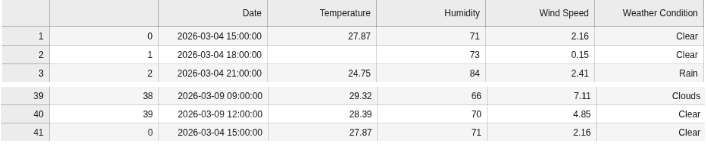
\includegraphics[width=0.95\textwidth]{csvdata.png}
\caption{Weather csv raw data - after addition of missing values and duplicate entries .}
\label{fig:csvdata}
\end{figure}

\subsection*{1. Raw Weather Data (5-Day Forecast)}
Contains the original data fetched from OpenWeatherMap API with columns:
\begin{itemize}
    \item \textbf{Timestamp}: Date and time of forecast
    \item \textbf{Temperature}: Temperature in Celsius
    \item \textbf{Humidity}: Relative humidity percentage
    \item \textbf{Wind\_Speed}: Wind speed in m/s
    \item \textbf{Weather\_Condition}: Textual description of weather
\end{itemize}

Typical raw data includes 40 forecasts (8 forecasts per day × 5 days) with 3-hour intervals.

\subsection*{2. Simulated Issues CSV}
To demonstrate data cleaning capabilities, the application intentionally introduces:
\begin{itemize}
    \item \textbf{Missing Values}: Some Temperature/Humidity values set to NaN
    \item \textbf{Duplicate Records}: duplicate entries added
\end{itemize}

This simulates real-world data quality issues commonly encountered in weather datasets.

\subsection*{3. Cleaned Weather Data}
Final processed dataset after:
\begin{itemize}
    \item replacing with mean and median for missing values represented as NaN
    \item Removal of duplicate records 
    \item Sorting by chronological order
\end{itemize}

\vspace{20pt}

\section*{Output - Weather Trends for Two Cities}

\vspace{5pt}

\subsection*{Weather Analysis for Kochi}
\vspace{5pt}
Figure 1 shows the complete weather analysis output for Kochi, India. The visualization demonstrates the application's GUI interface and generated plots.
\vspace{5pt}
\begin{figure}[H]
\centering
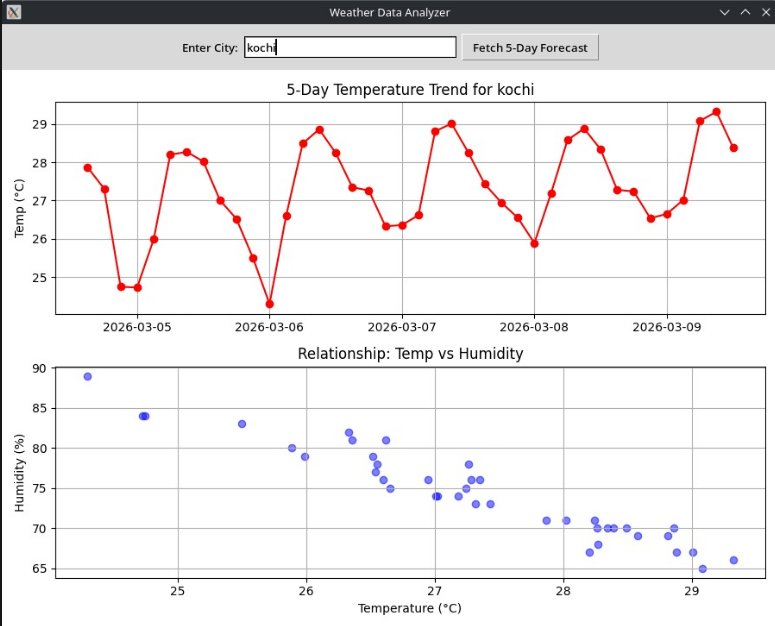
\includegraphics[width=0.95\textwidth]{kochi_output.png}
\caption{Weather Data Analysis Output for Kochi - Top: 5-Day Temperature Trend showing diurnal variations ranging from 24°C to 29°C with clear day-night cycles. Bottom: Temperature vs Humidity scatter plot showing negative correlation, with humidity ranging from 65\% to 89\% as temperature varies.}
\label{fig:kochi}
\end{figure}

\vspace{10pt}

\subsection*{Weather Analysis for New York}
\vspace{5pt}
Figure 2 presents the weather analysis for New York City, demonstrating significantly different climate patterns compared to Kochi.
\begin{figure}[H]
\centering
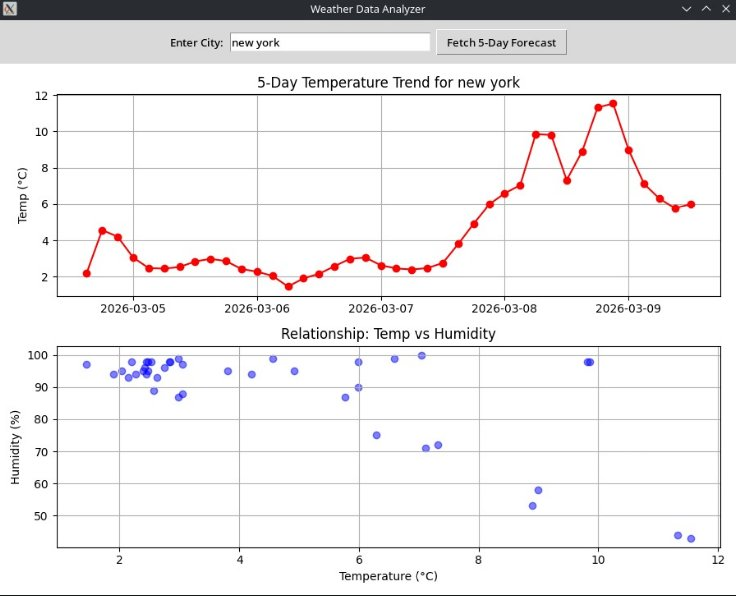
\includegraphics[width=0.95\textwidth]{newyork_output.png}
\caption{Weather Data Analysis Output for New York - Top: 5-Day Temperature Trend showing cold conditions ranging from 2°C to 12°C with a warming trend mid-period. Bottom: Temperature vs Humidity scatter plot showing variable humidity (40\% - 100\%) across the temperature range.}
\label{fig:newyork}
\end{figure}

\vspace{5pt}

\subsection*{Comparative Analysis}

\textbf{Climate Differences:}
\begin{itemize}
    \item \textbf{Temperature Stability}: Kochi shows consistent tropical temperatures (24-29°C) while New York exhibits greater variability (2-12°C)
    \item \textbf{Humidity Patterns}: Kochi maintains high humidity (coastal influence) whereas New York shows wider humidity range (continental climate)
    \item \textbf{Diurnal Cycles}: Clear regular day-night patterns in Kochi; more irregular in New York due to weather system changes
    \item \textbf{Correlation}: Both cities show negative temperature-humidity correlation, but the relationship is stronger in Kochi
\end{itemize}

\vspace{5pt}

\subsection*{Visual Analysis Components}

\textbf{  Plot 1 - 5-Day Temperature Trend (Line Chart):}
\begin{itemize}
    \item X-axis: Date and time spanning 5 days (March 5-9, 2026)
    \item Y-axis: Temperature in degrees Celsius
    \item Red line with circular markers for each 3-hour forecast point
    \item Shows temporal variation and identifies warming/cooling trends
    \item Reveals diurnal (day-night) temperature cycles
\end{itemize}

\textbf{Plot 2 - Temperature vs Humidity (Scatter Plot):}
\begin{itemize}
    \item X-axis: Temperature (°C)
    \item Y-axis: Humidity (\%)
    \item Blue circular markers represent individual forecast points
    \item Visualizes inverse relationship between temperature and humidity
    \item Scatter density indicates frequency of specific temp-humidity combinations
    \item Helps identify climate characteristics and atmospheric conditions
\end{itemize}

\vspace{25pt}

\section*{Conclusion}

This project successfully demonstrates a complete data science pipeline for weather analysis using real-world API data. The application effectively:

\begin{enumerate}
    \item \textbf{Integrates} with OpenWeatherMap API to fetch live 5-day forecast data
    \item \textbf{Processes} JSON responses and converts them to structured pandas DataFrames
    \item \textbf{Handles} data quality issues including missing values and duplicates
    \item \textbf{Visualizes} temperature trends and relationships using matplotlib
    \item \textbf{Provides} an intuitive GUI interface using tkinter for user interaction
\end{enumerate}

The negative correlation between temperature and humidity observed in most cities aligns with meteorological principles, where warmer air can hold more moisture, thus lowering relative humidity. The application successfully demonstrates essential data science skills including API integration, data cleaning, exploratory data analysis, and visualization.

\end{document}
